\chapter{Packaging and Tests under High Pressure}
\label{4}
In this chapter, packaging of both the chip housing and the test setup is presented. To start with, the packaging of the test setup is presented and an array of pressure accumulators is used, to increase stored fluid volume over the single canister shown in \autoref{3_6}. Then a preliminary chip housing design without integrating the NF membrane is introduced, followed by the second housing design which is improved based on the first design. The final housing design provides the possibility to integrate NF membrane. Therefore the positions of the inlet and outlet interfaces are changed and an additional supporting plate is introduced as the mechanical carrier of the NF membrane. At last the pressure and leakage test results and some calculation with respect to the flow parameters in the microchannel are presented.

\section{Packaging of the Test Setup}
\label{4_1}
In \autoref{3_6} the design of the test setup is presented. Since the system will be pressurized up to 10bar, all the connection interfaces and tubes should be able to withstand such high pressure. Therefore the adapters and connectors connecting to the pressure accumulator are made of metal (either brass or stainless steel (SS)). The chip housing is connected to this test setup by adapters and fittings made of PEEK and ETFE tubes which are designed for high pressure applications (up to 69bar). \autoref{figure4_1} shows the schematic design of all the connections and \autoref{figure4_2} shows the real packaging of the test setup and \autoref{table4_1} gives the name of the used parts, their material and the maximum pressure they can withstand.\\
\clearpage

\begin{figure}[h]%
\centering
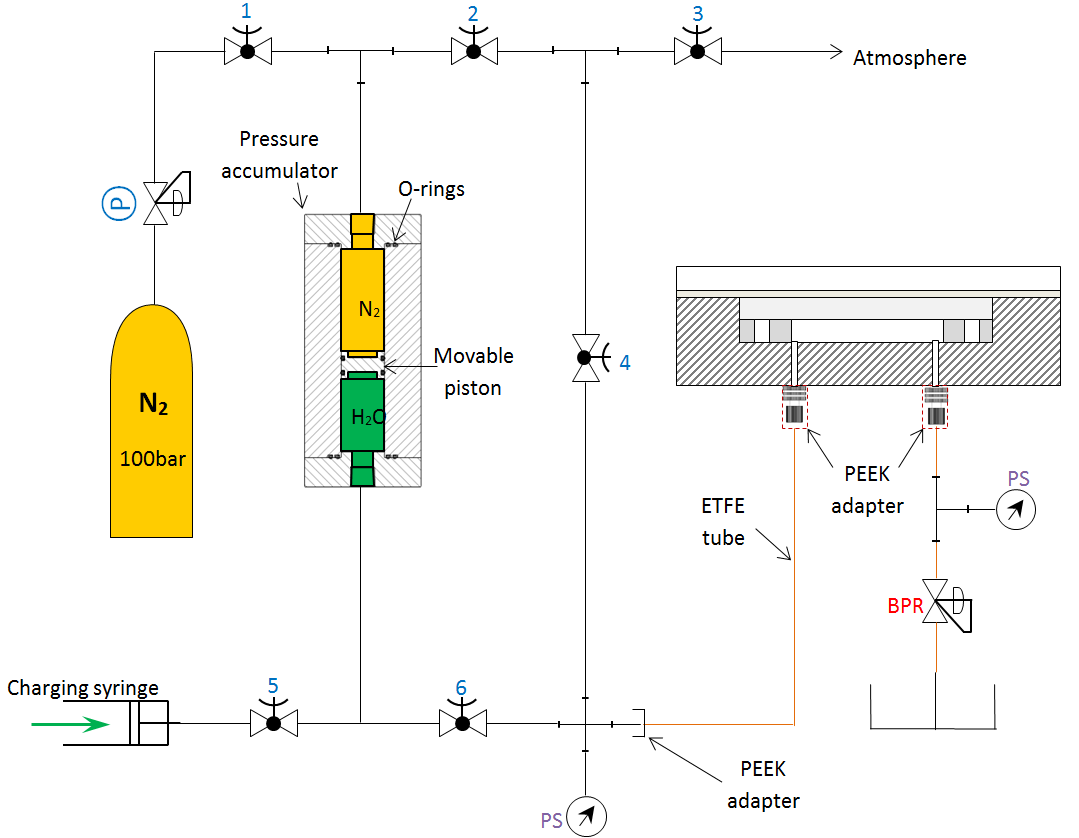
\includegraphics[width=0.82\textwidth]{figures/packagingandtestunderhighpressure/figure4_1}%
\caption{Schematic design of the test setup packaging with housing design 2 introduced in \autoref{3_5_2}.}%
\label{figure4_1}%
\end{figure}

\begin{table}[!h]
    \centering
    \caption{Used parts and their material and maximum working pressure}
    \begin{longtable}{l|l|l|l|l}
    \toprule
    No. & Name & Material & Pressure (bar) & Supplier \\
    \midrule
    1 & Needle valve & Brass & 206 & Swagelok \\
    2 & Plug valve & Brass & 206 & Swagelok \\
    3 & Tee & Brass & 248 & Swagelok \\
    4 & Cross & Brass & 248 & Swagelok \\
    5 & Tube fitting & Brass & 275 & Swagelok \\
    6 & Tubing & SS & 351 & Swagelok \\
    7 & Tube fitting & Brass & 227 & Swagelok \\
    8 & Connector & Brass & 227 & Swagelok \\
    9 & Connector & SS & 551 & Swagelok \\
    10 & Connector & Brass & 275 & Swagelok \\
    11 & Fitting & Brass & 275 & Swagelok \\
    12 & Pressure sensor &   & 0-250 & Gems \\
    13 & Adapter & PEEK & 69 & IDEX \\
    14 & Tube fitting & PEEK & 414 & IDEX \\
    15 & Tubing & ETFE & 207 & IDEX \\
    \bottomrule
    \end{longtable}
    \label{table4_1}
\end{table}
\clearpage

\begin{figure}[!h]%
\centering
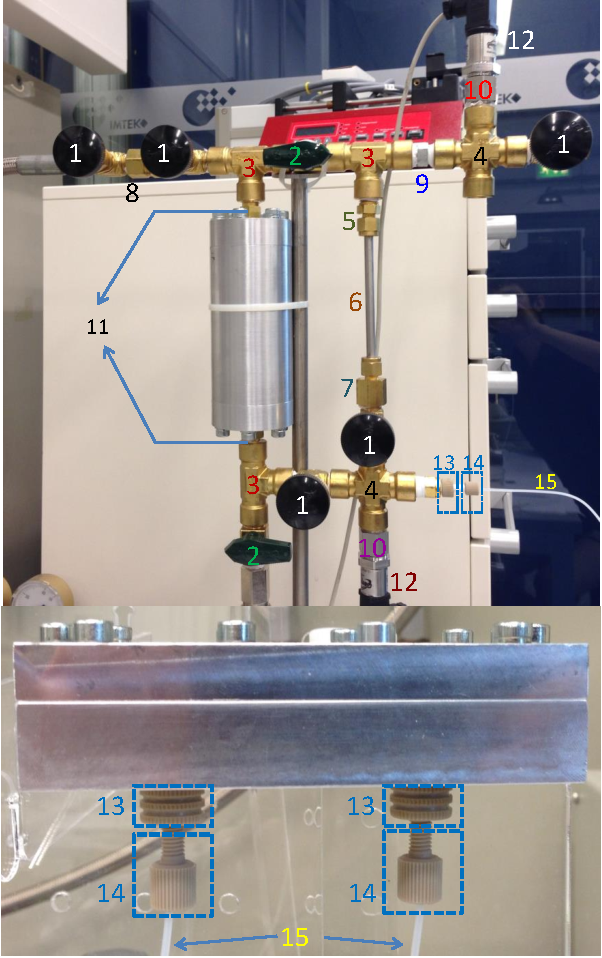
\includegraphics[width=0.6\textwidth]{figures/packagingandtestunderhighpressure/figure4_2}%
\caption{Practical packaging of the test setup and connection to the chip housing.}%
\label{figure4_2}%
\end{figure}

\autoref{figure4_3} shows the dimensions of the interior space of the pressure accumulator. The total usable volume that can be loaded is calculated to be 34.9mL according to these dimensions. However, such volume is not enough for continuous long-time (at least 30min) flow test since the volume flow rate is around 5mL/min as initial tests indicated. Therefore the pressure accumulator is redesigned to a canister array which contains six canisters instead of only one canister that was used before. The total available volume is expanded to about 210mL. \\

In the new design the six canisters stand on a holder. All the connectors, tube fittings and valves are made of brass and the metal tube is made of stainless steel. Therefore the maximum pressure this system can withstand is more than 200bar and this ensures the safety since the test in this thesis work is around 10bar. \autoref{figure4_4} shows the design and connection of the canister array.\\

\begin{figure}[ht]%
\centering
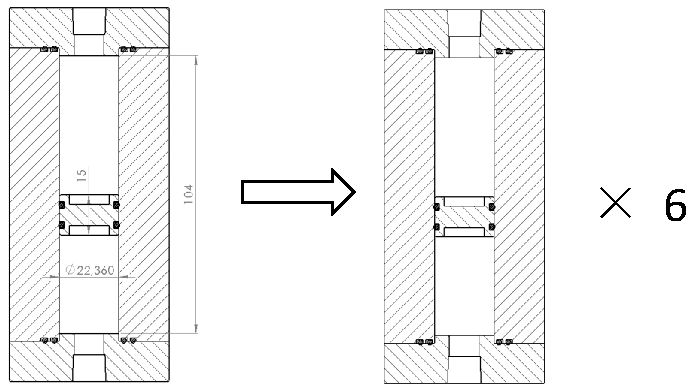
\includegraphics[width=0.5\textwidth]{figures/packagingandtestunderhighpressure/figure4_3}%
\caption{Dimensions of the pressure accumulator and the canister array.}%
\label{figure4_3}%
\end{figure}

\begin{figure}[ht]%
\centering
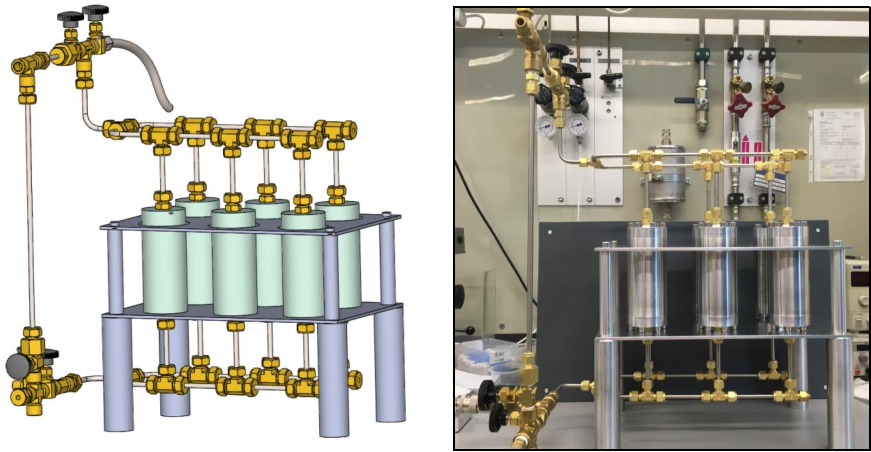
\includegraphics[width=1\textwidth]{figures/packagingandtestunderhighpressure/figure4_4}%
\caption{Design and connection of the canister array.}%
\label{figure4_4}%
\end{figure}
\clearpage


\section{Packaging and Pressure Test of the Microfluidic Platform Housing}
\label{4_2}
\subsection{Packaging Requirements}
\label{4_2_1}
Since the goal of this thesis work is to design a reusable and resealable microfluidic platform, the first task is to design a good packaging interface that fulfills the following requirements: reusability, resealability, easy manipulation, flexibility and fast connectivity. Besides, because this microfluidic platform is supposed to work under high pressure, it must provide reliable sealing (no leakage at high pressures) and mechanical stability (able to work at high pressures). Since the microfluidic platform should be assembled and disassembled for many times in order to test with different microchannel designs and different NF membranes with the same chip, the packaging must be adhesive-free as well.\\

One other important specification is the ability to have good visual access to the microchannel inside the housing. This is critical to the microfluidic platform because direct observation of the bacteria adhesion to the NF membrane surface is desired. A live monitoring of the bacteria is not only helpful to characterize the adhesion features under specific flow conditions, but also provides information about how to change the real-time flow conditions to control the adhesion heading for a certain direction (similar to closed-loop control). 

\subsection{Packaging and Pressure Test of Different Chip Housing Design}
\label{4_2_2}
\noindent \textit{Packaging of the housing design 1}\\

\begin{figure}[h]%
\centering
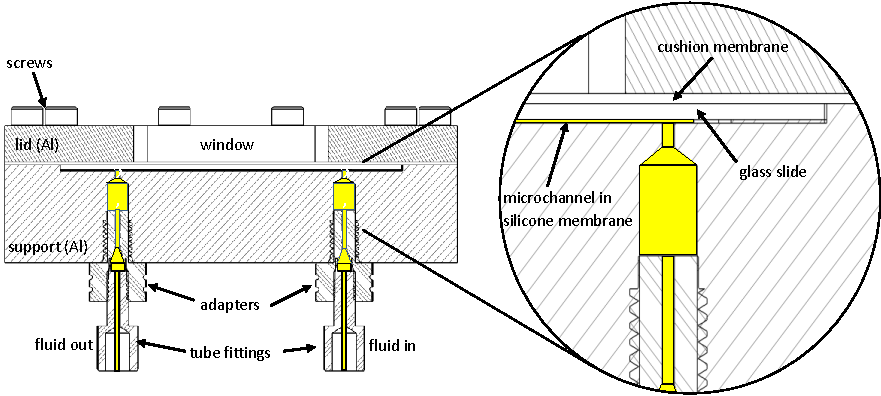
\includegraphics[width=0.95\textwidth]{figures/packagingandtestunderhighpressure/figure4_5}%
\caption{Schematic of the housing assembly (design 1).}%
\label{figure4_5}%
\end{figure}

The first design consists of an aluminum housing, glass slide with silicone membrane which has built-in microchannel, a cushion silicone membrane, macro-to-micro adapters and 12 screws (M4).\\

\begin{figure}[h]%
\centering
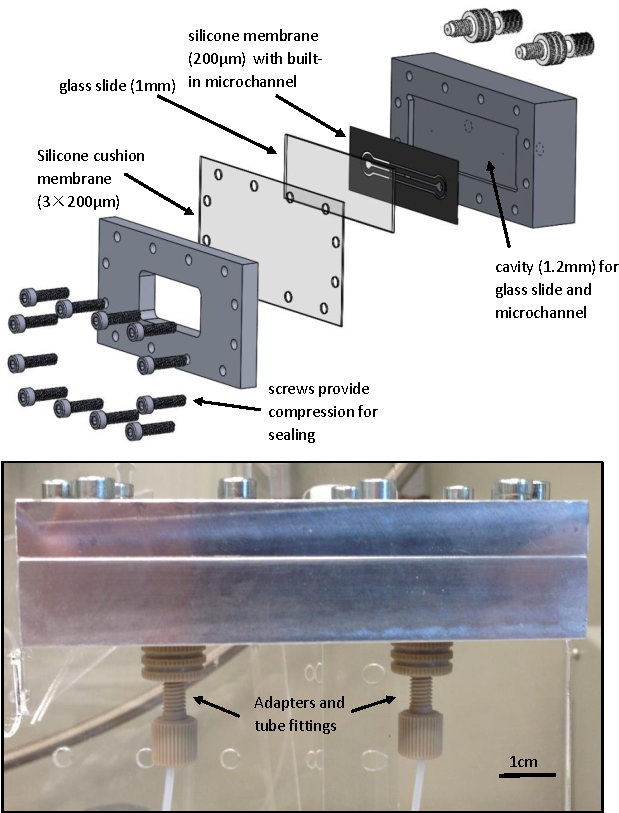
\includegraphics[width=0.7\textwidth]{figures/packagingandtestunderhighpressure/figure4_6}%
\caption{Explosion view of the housing assembly and packaged housing assembly.}%
\label{figure4_6}%
\end{figure}

\autoref{figure4_5} shows the schematic of the housing assembly. The inlet and outlet interfaces are at the bottom of the support plate, coupled with adapters and tube fittings from IDEX. The fluid enters the microchannel through an orifice which has a diameter of 1mm and this orifice is sealed by the glass slide and the surrounding silicone gasket. The connecting tube is made of ETFE and has an out diameter of 1/16inch (1.5875mm) and inner diameter of 0.02inch (0.5mm). A cavity in the support plate is designed for the location and the alignment of the glass slide and silicone membrane. There is an aperture machined in the center of the lid and it works as a window for visual access to the microchannel. \\

Before the packaging is started, the cavity in the aluminum support plate, the silicone membrane, the glass slide and the silicone cushion membrane need to be cleaned by ethanol to remove the dust at surfaces as much as possible.  Then the microchannel and the carrier glass slide are placed into the cavity in the support plate and are aligned to the cavity, after which three layers of cushion silicone membrane (3$\times$200$\mu$m) are placed in between the lid and the support plate in order to prevent damaging the glass slide by avoiding direct metal-glass contact since glass is rigid and fragile material. Finally the lid is joined to the support plate by twelve M4 screws and four edges of the glass slide are compressed by the lid as shown in \autoref{figure4_6}.\\


\noindent \textit{Test results and evaluation of housing design 1}\\

\begin{figure}[!b]%
\centering
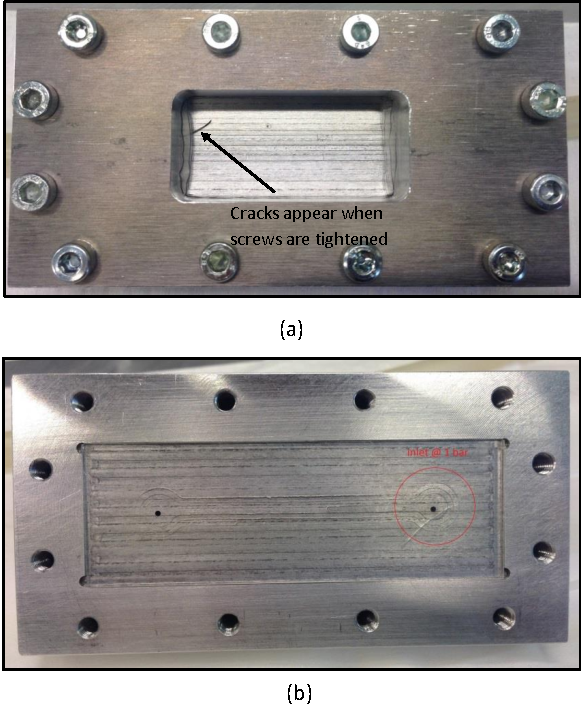
\includegraphics[width=0.6\textwidth]{figures/packagingandtestunderhighpressure/figure4_7}%
\caption{(a) Cracks appeared during the packaging. (b) Crack appeared when pressurized up to 1bar.}%
\label{figure4_7}%
\end{figure}

Before pressure test all the screws are tightened. Then the outlet interface is plugged to hold the pressure inside the microchannel. The microchannel should withstand each test pressure for at least 10min in order to test the long-term stability. Furthermore, any leakage will also be checked.\\

The screws were tightened stepwise with increasing torque, using a star pattern to ensure loading remained as evenly distributed as possible. By tightening the screws different torque values were tried (2N$\cdot$m, 1.5N$\cdot$m, 1N$\cdot$m). However, as shown in \autoref{figure4_7} (a), cracks appeared in the glass slide when the torque is set to 2N$\cdot$m and 1.5N$\cdot$m. Even though the glass slide remained intact at 1N$\cdot$m tightening torque, it broke at the inlet interface when the pressure reached 1bar as presented in \autoref{figure4_7} (b). \\

The cracks appeared in the glass slide during tightening the screws because of the uneven compression force to the glass slide. Since the center part of the glass slide is not covered by the aluminum lid because of the viewing window, the compression force distributes only to the four edges of the glass slide, leading to an uneven force distribution. Therefore even no cracks appear during assembling the housing, it will bring more risk when it is working under high pressure.\\

Another drawback of this housing design is the limited view of the microchannel. Since the viewing window in the lid is relatively small, the inlet and outlet interfaces are covered by the lid. Therefore for a better visual access to the microchannel the lid should be redesigned.\\

\noindent \textit{Packaging of the housing design 2}\\

\begin{figure}[!b]%
\centering
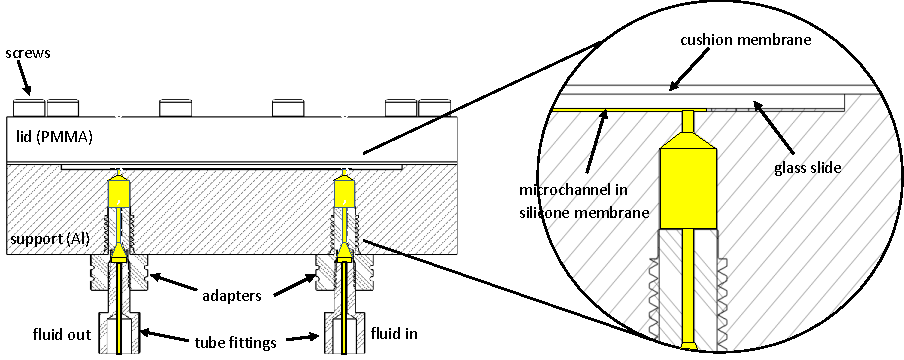
\includegraphics[width=1\textwidth]{figures/packagingandtestunderhighpressure/figure4_8}%
\caption{Schematic of the housing assembly (design 2).}%
\label{figure4_8}%
\end{figure}

In the second chip housing design the aluminum lid is replaced by a PMMA lid while the other parts remain the same. Since PMMA has excellent optical transparency, the whole microchannel can be viewed from the top side. Furthermore, no window aperture is needed in the lid so that the PMMA lid is in full contact with the glass slide, which provides a homogeneous force distribution to the glass slide surface. \autoref{figure4_8} shows the schematic of the chip housing assembly, the packaging procedure is the same to the first design. The silicone microchannel, the glass slide together with the silicone cushion membrane and the PMMA lid need to be cleaned before packaging because any uneven points at the surfaces can cause failure of the glass slide, and this damage can be amplified especially by the high pressure.\\

\noindent \textit{Test results and evaluation of housing design 2}\\

The torque applied to the screws was set to 1.2N$\cdot$m and no cracks presented during the packaging of the housing. This is because the force distribution is even at the glass slide surface. Then the pressure was applied to the microchannel gradually, starting from 1bar with a step of 0.2bar.  One crack appeared at the outlet interface when the pressure reached 3.4bar as shown in \autoref{figure4_9} (a). 

\begin{figure}[!h]%
\centering
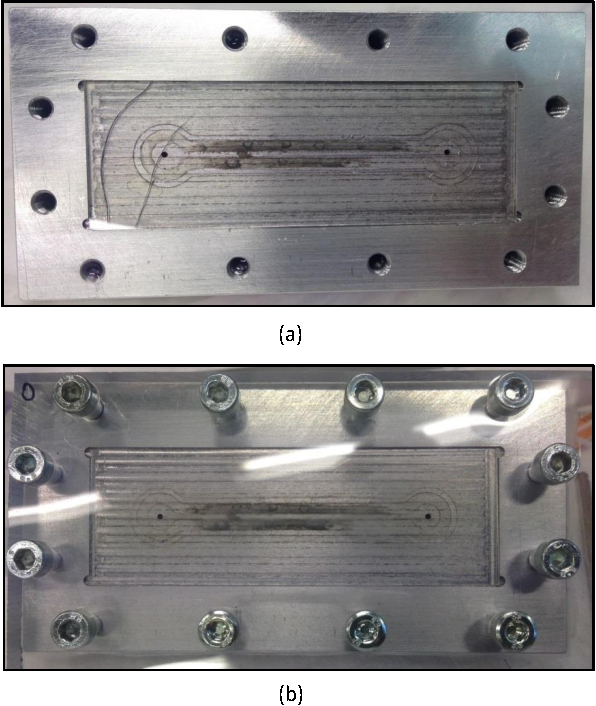
\includegraphics[width=0.6\textwidth]{figures/packagingandtestunderhighpressure/figure4_9}%
\caption{(a) Crack appeared at 3.4bar with screw torque of 1.2N$\cdot$m. (b) No crack appeared when loaded to 8bar with screw torque of 1N$\cdot$m.}%
\label{figure4_9}%
\end{figure}

Then the torque applied to the screws was lowered to 1N$\cdot$m in the next experiment. Likewise, no cracks in the glass slide presented during packaging. The microchannel was pressurized up to 8bar for two times and for each time it stayed at 8bar for 30min. Finally the glass slide remained intact as shown in \autoref{figure4_9} (b). This indicates that silicone microchannel with glass slide as its mechanical carrier can seal well by compression and is able to work under high pressure.

\noindent \textit{Packaging of the housing design 3}\\

\begin{figure}[h]%
\centering
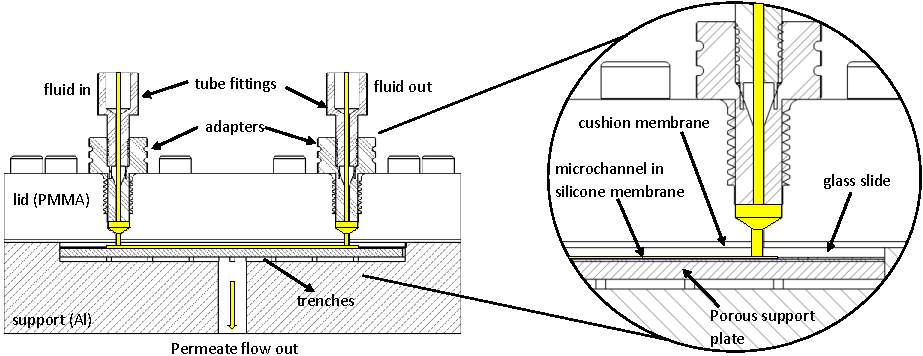
\includegraphics[width=1\textwidth]{figures/packagingandtestunderhighpressure/figure4_10}%
\caption{Schematic of the housing assembly (design 3).}%
\label{figure4_10}%
\end{figure}

In the third housing design the NF membrane is taken into account. Since the NF membrane should be intact to ensure valid filtration, the inlet and outlet interfaces are placed in the PMMA lid. In this case the permeate flow is introduced by the filtration performance of the NF membrane. Therefore a porous support plate is placed under the NF membrane and several trenches are designed underneath the porous support plate to collect the permeate flow. A single layer of 600$\mu$m silicone cushion membrane is placed in between the lid and the housing support instead of three layers of 200$\mu$m thick membranes.  \autoref{figure4_10} shows the schematic of the chip housing assembly. The packaging procedure is the same to the prior designs.\\

\noindent \textit{Test results and evaluation of housing design 3}\\

For pressure and leakage test the NF membrane is not initially applied. A piece of stainless steel of the same thickness was placed instead of the NF membrane. \autoref{figure4_11} shows the packaged housing with microchannel integrated inside. Likewise, no crack presented when the tightening torque is 1N$\cdot$m and it worked stably under high pressure (8bar).\\
\clearpage

\begin{figure}[h]%
\centering
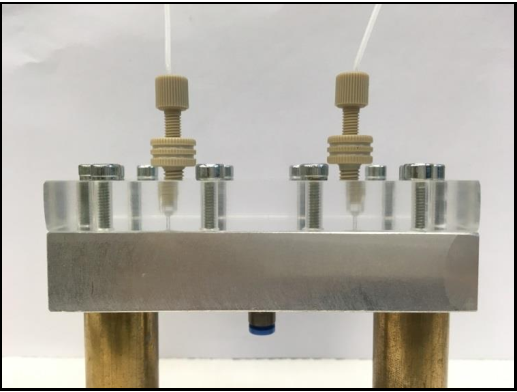
\includegraphics[width=0.6\textwidth]{figures/packagingandtestunderhighpressure/figure4_11}%
\caption{Packaged housing of design 3.}%
\label{figure4_11}%
\end{figure}

\section{Hydrodynamic Characterization of the Microchannel}
\label{4_3}
As presented in \autoref{4_2}, housing design 3 provides a stable performance working under high pressure and also offers the possibility to integrate NF membrane into the housing. Therefore the hydrodynamic characterization tests of the microchannel are done with housing design 3 and \autoref{figure4_12} shows the schematic of the test setup.\\

Two pressure sensors are integrated to the flow path to measure the fluid pressure before it enters the microchannel and after it leaves the microchannel. In the following tests the total pressure drop is achieved by calculating the pressure difference measured by these two pressure sensors. Therefore this total pressure drop is consisted of the pressure drop in the tube through which fluid enters the chip housing, the pressure drop in the microchannel and the pressure drop in the tube which connects the outlet of the chip housing and the second pressure sensor. The pressure sensor is a current output transducer which has a measuring range from 0 to 250bar. \\
\clearpage

\begin{figure}[h]%
\centering
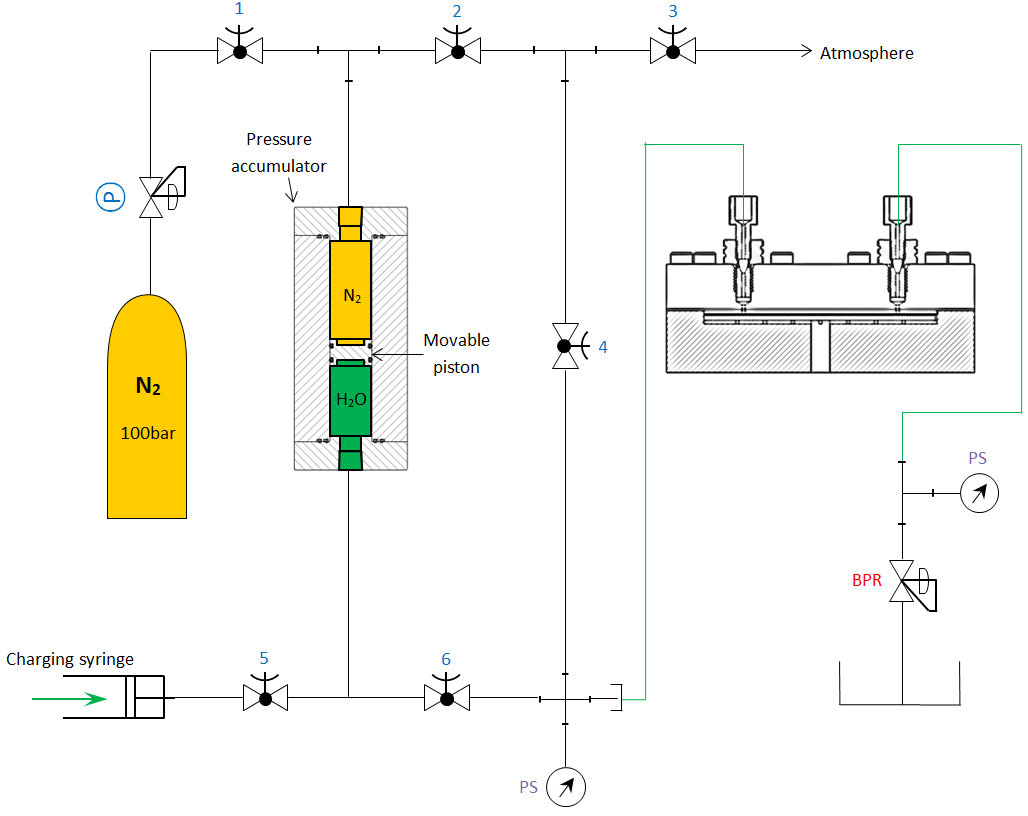
\includegraphics[width=0.85\textwidth]{figures/packagingandtestunderhighpressure/figure4_12}%
\caption{Schematic of the test setup with housing design 3.}%
\label{figure4_12}%
\end{figure}

\subsection{Calibration of the Pressure Sensor}
\label{4_3_1}
The pressure sensor is calibrated before use. Since the output of the pressure sensor is current with respect to the pressure and the available data acquisition (DAQ) NI-6008 USB device in our lab can only measure analog voltage, a resistor of 1k$\ohm$ is connected to the pressure sensor as shown in \autoref{figure4_13}. The pressure sensor is powered by a voltage source with a voltage of 30V. In this way the output current is converted to voltage and this voltage is estimated to be in the range of 4V to 5V. Since the analog-to-digital converter (ADC) in the DAQ device might also consume part of current for the measurement of the voltage between both sides of the resistor, possible disturbance might be introduced if the DAQ device is connected directly in parallel to the resistor and takes part of the current that should flow through the resistor. Therefore, an operational amplifier which is connected as a voltage follower is placed as a barrier between the resistor and the DAQ module since it consumes nearly no current at the input side because of its large input resistance. Moreover, the voltage between the two sides of the resistor is precisely transferred to the DAQ module since the very low output resistance of the operational amplifier does not consume this voltage. The sample rate of the DAQ module is set to 1k, indicating that 1000 samples will be sent to the computer via USB cable within one second. The Labview program in the computer receives the data and calculates the average value of every 1000 pressure data, resulting in a relatively more stable and precise output display in the user interface. Two channels of analog voltage input port are used for the two pressure sensors. 

\begin{figure}[h]%
\centering
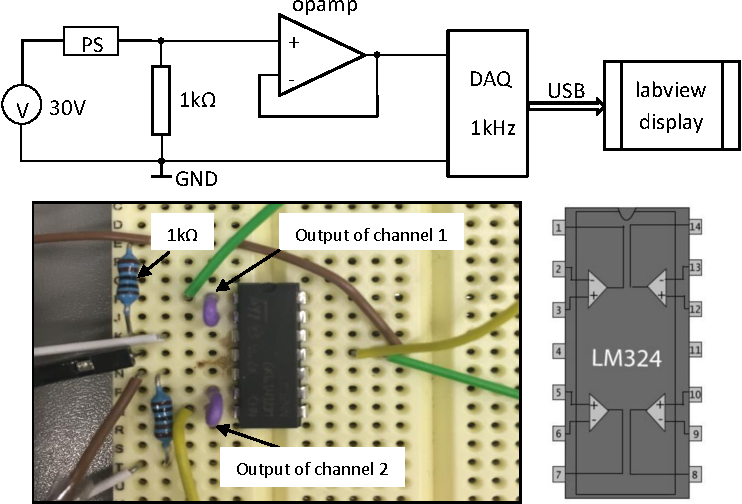
\includegraphics[width=0.9\textwidth]{figures/packagingandtestunderhighpressure/figure4_13}%
\caption{Electrical connections for pressure measurement}%
\label{figure4_13}%
\end{figure}

The calibration pressure starts from 1 bar to 7bar with a step of 0.5bar. The measured voltage corresponding to the pressure is listed in \autoref{table4_2}. Based on this acquired data linear regression is done to figure out the linear relation between pressure and measured voltage. \autoref{figure4_14} shows the results graph of the linear regression and the linear equation is given below:

\begin{table}[!h]
    \centering
    \caption{Measured voltage and the corresponding pressure}
    \begin{tabular}{cc}
    \toprule
    Pressure (bar) & Measured Voltage (V) \\
    \midrule
    1 & 4.05\\
    1.5 & 4.09\\
    2 & 4.11\\
    2.5 & 4.15\\
    3 6 & 4.18\\
    3.5 & 4.21\\
    4 & 4.24\\
    4.5 & 4.27\\
    5 & 4.31\\
    5.5 & 4.34\\
    6 & 4.37\\
    6.5 & 4.40\\
    7 & 4.44\\
    \bottomrule
    \end{tabular}
    \label{table4_2}
\end{table}

\begin{figure}[!h]%
\centering
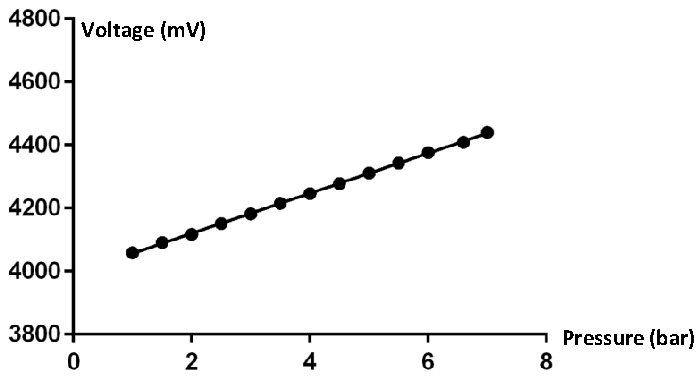
\includegraphics[width=0.6\textwidth]{figures/packagingandtestunderhighpressure/figure4_14}%
\caption{Linear regression of the voltage and pressure.}%
\label{figure4_14}%
\end{figure}

\begin{equation}
    V=63.45 \cdot P+3993
    \label{equation4_1}
\end{equation}

\begin{equation}
    R^2=0.9997
    \label{equation4_2}
\end{equation}

where V is the measured voltage (mV) and P is the corresponding pressure (bar). Since the coefficient of determination, $R^{2}$, is very close to 1, the linearity between voltage and pressure is good enough. According to the \autoref{equation4_1} pressure can be calculated with respect to the measured voltage as shown in \autoref{equation4_3}. For the following tests the pressure (P) is calculated according to \autoref{equation4_3} by Labview and saved.

\begin{equation}
    P=\frac{V-3993}{63.45}
    \label{equation4_3}
\end{equation}

\subsection{Cross Flow Rate Measurement}
\label{4_3_2}

\begin{figure}[!b]%
\centering
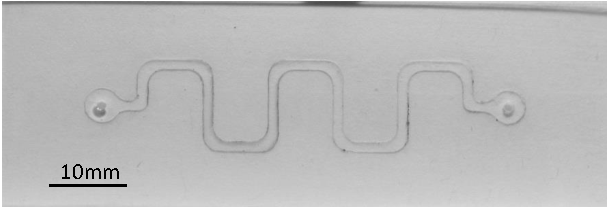
\includegraphics[width=0.6\textwidth]{figures/packagingandtestunderhighpressure/figure4_15}%
\caption{Microchannel geometry under test.}%
\label{figure4_15}%
\end{figure}

To characterize the hydrodynamic parameters of the microchannel, the cross flow rate under different pressures is measured and the pressure difference between the two pressure sensors is also calculated. \autoref{figure4_15} shows the microchannel geometry under test. No permeation flow is introduced and the NF membrane is replaced by a piece of steel sheet in this test.\\



The fluid loading in the system in this test is water. The flow rate is measured by recording the time for collecting 5mL water at the outlet interface after the back pressure regulator. \autoref{figure4_16} shows the pressure profile recorded by Labview, including the pressure data from the two pressure sensors and the pressure difference of the two pressure sensors. \autoref{table4_3} shows the measured pressures before and after the microchannel and the calculated volume flow rate:

\begin{figure}[ht]%
\centering
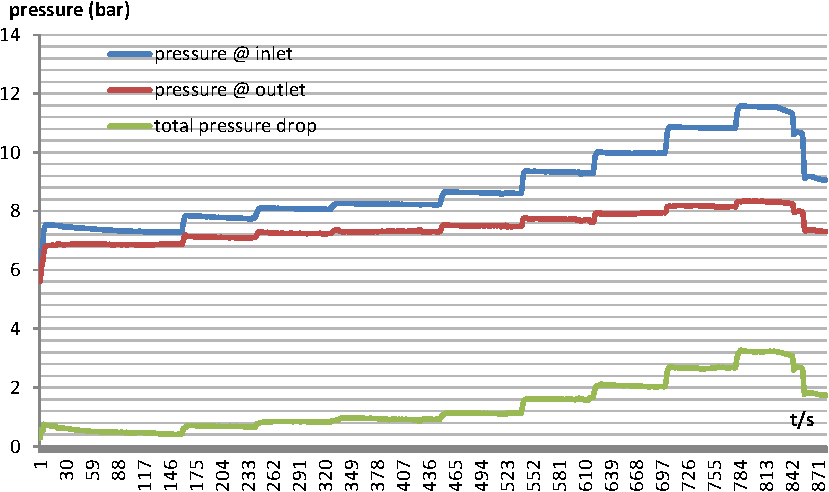
\includegraphics[width=0.8\textwidth]{figures/packagingandtestunderhighpressure/figure4_16}%
\caption{Recorded pressure data from Labview.}%
\label{figure4_16}%
\end{figure}

\autoref{figure4_17} shows the plot of total pressure drop and the flow rate in the channel versus the pressure at inlet interface. The flow rate in the channel shows good linearity with respect to the input pressure and this means the flow rate can be estimated by controlling the input pressure.\\
\clearpage

\begin{table}[!h]
    \centering
    \caption{Pressure data and corresponding volume flow rate.}
    \begin{tabular}{C{2.3cm} C{2.3cm} C{2.3cm} C{2.5cm} C{2.2cm}}
    \toprule
    Inlet Pressure (bar) & Outlet Pressure (bar) & Pressure Drop (bar) & Time for 5mL Collection (s) & Volume Flow Rate (mL/min) \\
    \midrule
    7.35 & 6.85 & 0.5 & 95 & 3.1579\\
    7.8 & 7.1 & 0.7 & 69 & 4.3478\\
    8.08 & 7.24 & 0.85 & 57 & 5.2632\\
    8.25 & 7.3 & 0.95 & 52 & 5.7692\\
    8.64 & 7.5 & 1.14 & 42 & 7.0588\\
    9.35 & 7.75 & 1.6 & 33 & 9.0909\\
    9.98 & 7.9 & 2.08 & 27 & 11.1111\\
    10.8 & 8.15 & 2.65 & 22 & 13.6364\\
    11.5 & 8.3 & 3.2 & 19 & 15.7894\\
    \bottomrule
    \end{tabular}
    \label{table4_3}
\end{table}

\begin{figure}[!h]
\centering
\subfigure{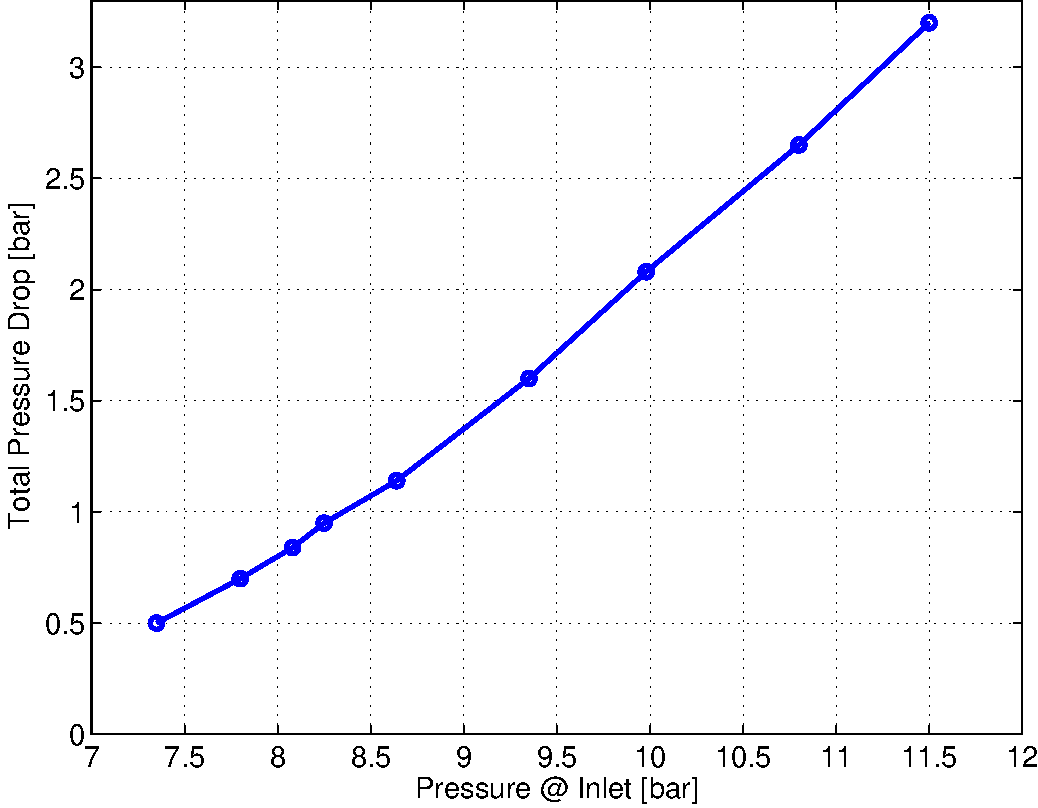
\includegraphics[width=0.48\textwidth]{figures/packagingandtestunderhighpressure/figure4_17a.pdf}}
\centering
\subfigure{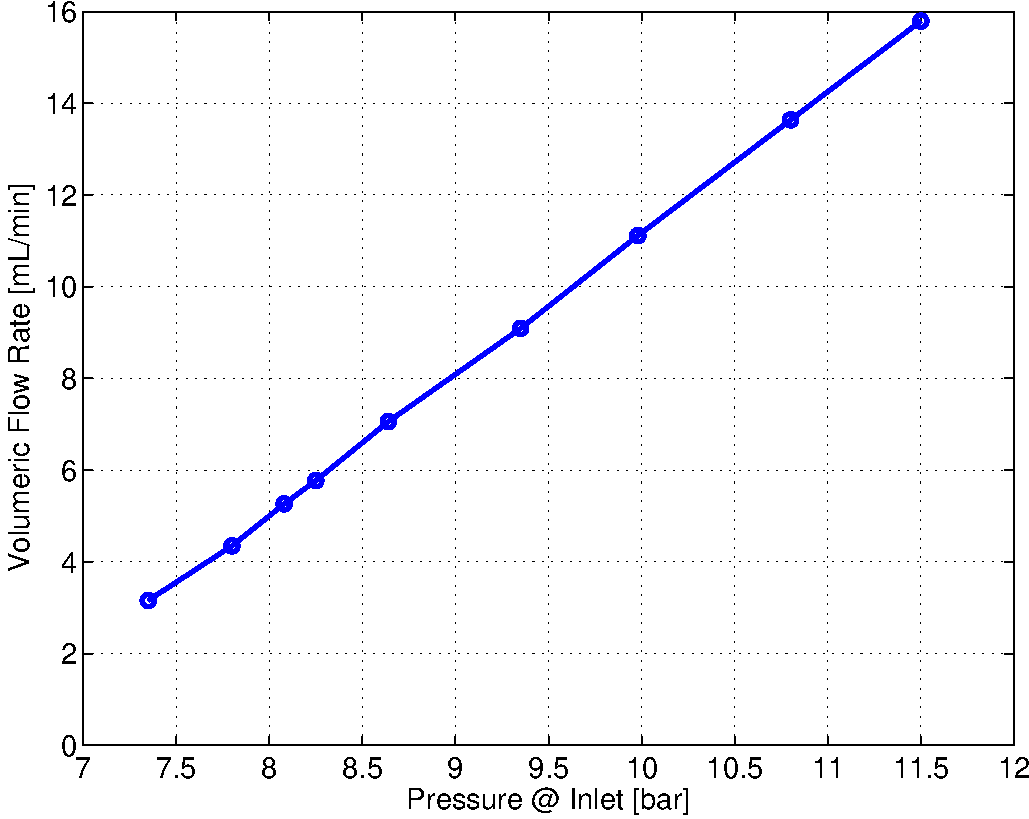
\includegraphics[width=0.48\textwidth]{figures/packagingandtestunderhighpressure/figure4_17b.pdf}}
\centering
\caption{(a) Total pressure drop versus pressure at inlet. (b) Volumetric flow rate in the microchannel versus total pressure drop.}
\label{figure4_17}%
\end{figure}

\noindent \textit{Fluidic system modeling}\\

As shown in \autoref{figure4_18} (a), there are three segments between the two pressure sensors: the tube through which fluid reaches the inlet of the chip housing, the microchannel in the housing and the tube connecting the outlet of the housing to the second pressure sensor. The pressure difference between the two pressure sensors therefore contains respective pressure drop in these three segments. An analogy to electrical circuits may be made, in which the total pressure drop is regarded as a voltage source while the flow rate is regarded as current. Likewise, each segment tube and the microchannel have their own fluidic resistances. \autoref{figure4_18} (b) presents the corresponding electric circuit representing this hydrofluidic system. \autoref{equation4_4} gives the Ohm's law in hydrodynamics:

\begin{equation}
    \Delta P=I_V\cdot R
    \label{equation4_4}
\end{equation}

In the equation above, $\Delta$P is the pressure drop measured by the two pressure sensors, $I_V$ is the volume flow rate which represents current in electric circuits and R is the fluidic resistance. For laminar flow in the tubes with circular cross-section the flow rate can be calculated according to Hagen-Poiseuille-Law \cite{hpequation}:

\begin{equation}
    I_V=\frac{\pi r^4}{8\eta} \frac{\Delta P}{l}
    \label{equation4_5}
\end{equation}

Where r is the inner diameter of the tube, $\eta$ is the dynamic viscosity of the fluid, $\Delta$P is the pressure drop and l is the length of the tube. Therefore the fluidic resistance of the tube is given by \autoref{equation4_6}:

\begin{equation}
    R_{circle}=\frac{8\eta l}{\pi R^4}
    \label{equation4_6}
\end{equation}

The dynamic viscosity of water at room temperature is given \cite{waterviscosity}:

\begin{equation}
    \eta (water)=890\times 10^{-6} Pa\cdot s
    \label{equation4_7}
\end{equation}

The fluidic resistance of rectangular cross-section microchannel under laminar flow is given by the following equation \cite{fuerstman2007pressure}:

\begin{equation}
    R_{rechtangle} = \frac{12\eta l}{WH^3}[1-\frac{192H}{\pi ^5 W}\tanh{(\frac{\pi W}{2H})}]^{-1}
    \label{equation4_8}
\end{equation}

Where W is the width of the channel and H is the height of the channel.

\begin{figure}[ht]%
\centering
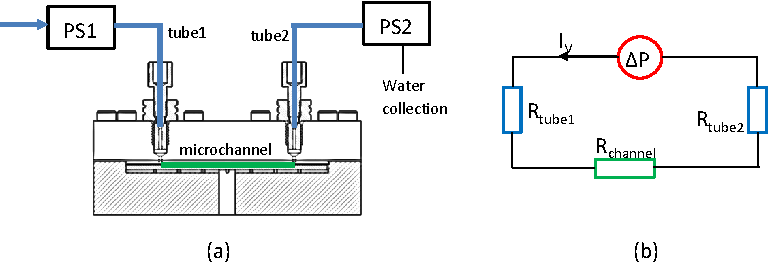
\includegraphics[width=0.9\textwidth]{figures/packagingandtestunderhighpressure/figure4_18}%
\caption{(a) Fluidic system under measurement. (b) Corresponding equivalent circuit.}%
\label{figure4_18}%
\end{figure}

\noindent \textit{Dimension of the tube and microchannel}\\

The total length of the tube is 1350mm and the inner diameter of the tube is 0.5mm. The total length of the silicone channel on the chip is 115mm. The cross-section of the channel is rectangular with a width of 1mm and a height of 0.2mm. Since the silicone microchannel is sealed by compression, it is estimated that a 5$\%$ error of the microchannel dimension might occur, meaning that the height of the microchannel might be compressed to the 95$\%$ of its original height and the width might also be compressed to the 95$\%$ of its original width.\\

With the dimensions of both the tube and the microchannel the Reynolds Number (Re) can be calculated according to the following equation:

\begin{equation}
    Re=\frac{\rho vD_H}{\eta}
    \label{equation4_9}
\end{equation}

Where $\rho$ is the density of water, v is the flow velocity and $D_H$ is the hydraulic diameter.

Since the volume flow rate is calculated as shown in \autoref{table4_3}, the pressure drop in the two segments of tubes can be calculated according to \autoref{equation4_5} and thus the experimental pressure drop in the microchannel can be figured out as the following equation shows:

\begin{equation}
    \Delta P_{total} = \Delta P_{tube1} + \Delta P_{channel} + \Delta P_{tube2}
    \label{equation4_10}
\end{equation}

Apart from that, the fluidic resistance of the microchannel can be calculated according to \autoref{equation4_8} and thus the theoretical pressure drop ($\Delta P_{T-channel}$) along the microchannel can also be calculated based on Equation 4.4:

\begin{equation}
    \Delta P_{T-channel} = I_V \cdot R_{channel}
    \label{equation4_11}
\end{equation}

$R_{channel}$ is the fluidic resistance of the microchannel calculated by \autoref{equation4_8} and $I_V$ is the flow in the microchannel.\\

The experimental pressure drop ($\Delta P_{E-channel}$) is also calculated by subtracting the pressure drop in tubes from the total pressure drop as shown in the following equation: 

\begin{equation}
    \Delta P_{E-channel} = \Delta P_{total} - \Delta P_{tube1} - \Delta P_{tube2}
    \label{equation4_12}
\end{equation}

The comparison of the theoretical pressure drop ($\Delta P_{T-channel}$) and experimental pressure drop ($\Delta P_{E-channel}$) along the microchannel are presented as shown in \autoref{table4_4} and the total pressure drop, the pressure drop in the tube and the pressure drop in the microchannel are plotted with respect to the volumetric flow rate as shown in \autoref{figure4_19}. \\

\begin{table}[!h]
    \centering
    \caption{Pressure drop in the tube, pressure drop in the microchannel (experimental and theoretical) and Reynolds Number in tube and microchannel with respect to the total pressure between pressure sensors.}
    \begin{tabular}{C{2.3cm}C{1.5cm}C{1.5cm}C{1.5cm}C{1.5cm}C{2cm}C{2cm}}
    \toprule
    $I_V$ (mL/min) & $\Delta P_{total}$ (bar) & $Re_{tube}$ &$\Delta P_{tube}$ (bar) & $Re_{channel}$ & $\Delta P_{E-channel}$ (bar) & $\Delta P_{T-channel}$ (bar) \\
    \midrule
    3.1579 & 0.50 & 221 & 0.4122 & 97 & 0.0878 & 0.0924\\
    4.3478 & 0.70 & 304 & 0.5676 & 134 & 0.1324 & 0.1272\\
    5.2632 & 0.85 & 368 & 0.6871 & 163 & 0.1629 & 0.1540\\
    5.7692 & 0.95 & 404 & 0.7531 & 178 & 0.1969 & 0.1688\\
    7.0588 & 1.14 & 494 & 0.9215 & 218 & 0.2185 & 0.2065\\
    9.0909 & 1.60 & 636 & 1.1868 & 281 & 0.4132 & 0.2660\\
    11.1111 & 2.08 & 778 & 1.4505 & 343 & 0.6295 & 0.3251\\
    13.6364 & 2.65 & 955 & 1.7801 & 421 & 0.8699 & 0.3990\\
    15.7894 & 3.20 & 1105 & 2.0612 & 488 & 1.1388 & 0.4620\\
    \bottomrule
    \end{tabular}
    \label{table4_4}
\end{table}


\begin{figure}[!h]
\centering
\begin{subfigure}
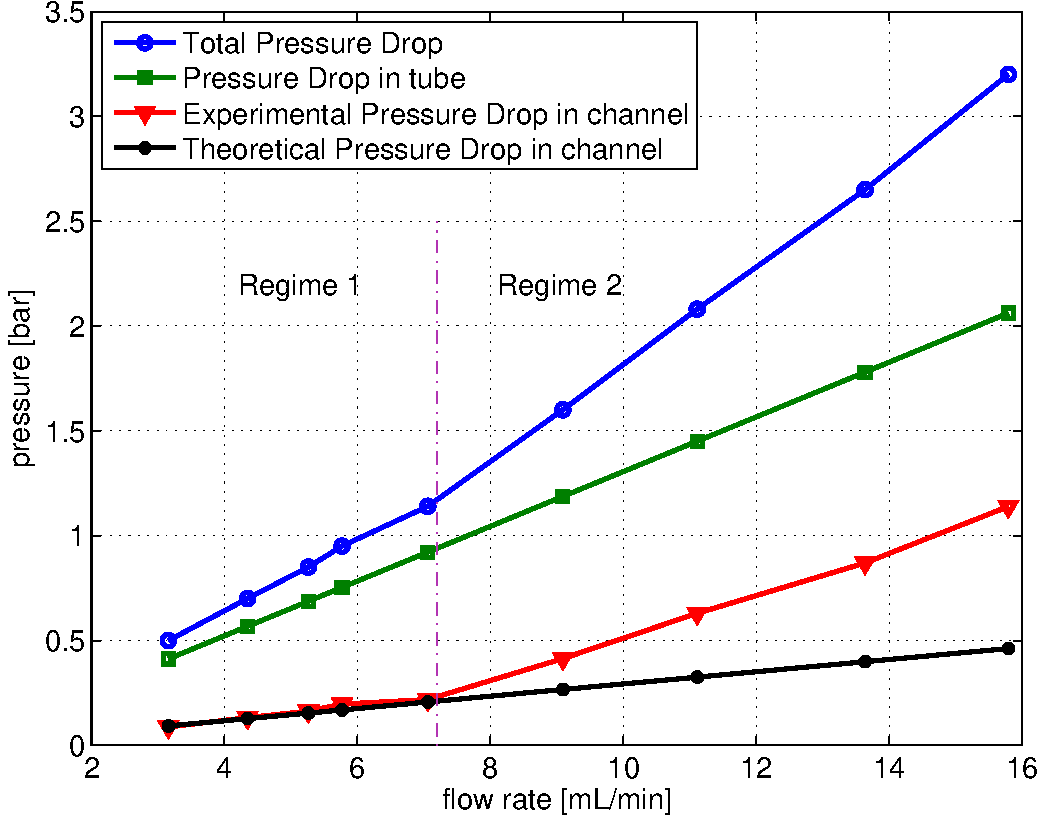
\includegraphics[width=0.48\textwidth]{figures/packagingandtestunderhighpressure/figure4_19a.pdf}
\end{subfigure}
\begin{subfigure}
{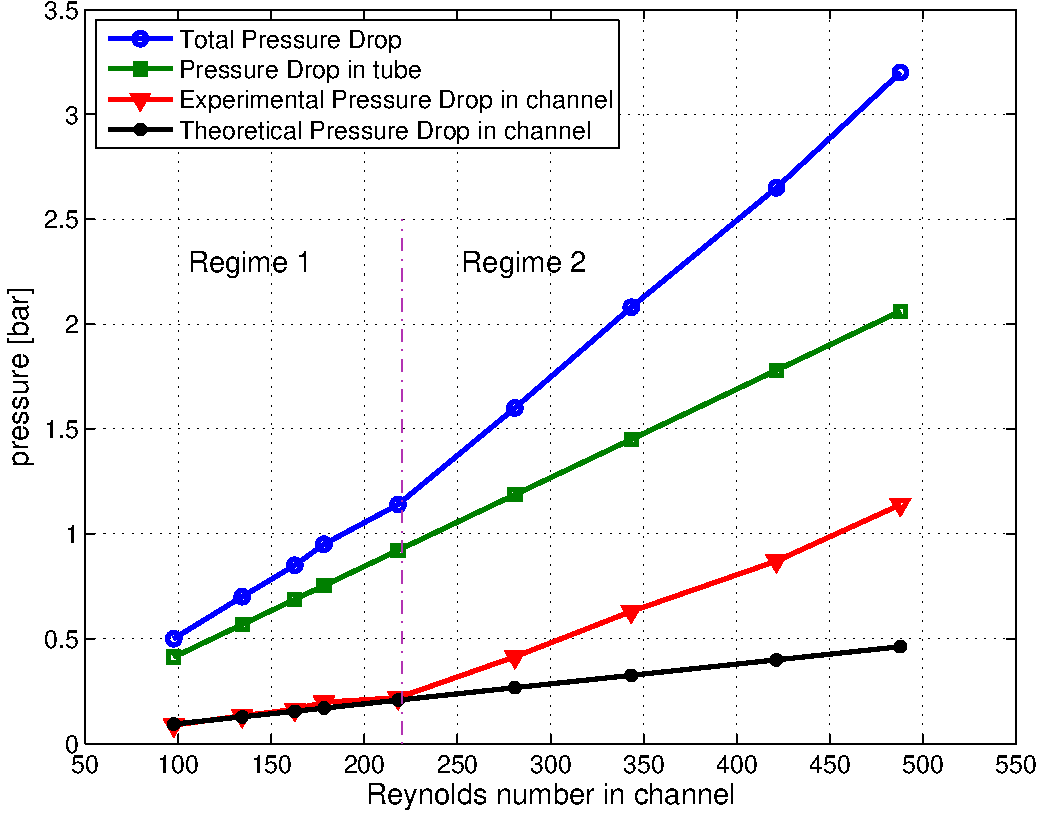
\includegraphics[width=0.48\textwidth]{figures/packagingandtestunderhighpressure/figure4_19b.pdf}}
\end{subfigure}
\caption{Total pressure drop, pressure drop in the tube and both experimental and theoretical pressure drop in the microchannel with respect to volumetric flow rate.}
\label{figure4_19}%
\end{figure}

When the flow rate in the tube and the microchannel is relatively high (higher than approximately 7.2mL/min), the corresponding Reynolds Number is also relatively larger than that in regime 1 and impact of the corners in the microchannel shown in \autoref{figure4_15} would be more significant due to the high flow rate, resulting in a more chaotic flow in the microchannel. Moreover, the inlet and outlet orifices are perpendicular to the inlet and outlet reservoirs as shown in \autoref{figure4_18} and this might also make a contribution to the chaotic flow in the microchannel. And these are perhaps the reasons why the gradient of the total pressure drop and the gradient of the experimental pressure drop in channel differ in these two regimes since Hagen-Poiseuille-Law is used to calculate the pressure drop of the fluid in laminar flow. When the flow is more laminar in Regime 1 and the impact from the microchannel geometry is less significant due to the low flow rate, the theoretically calculated pressure drop in the channel matches the experimental results well. For further studies the pressure loss due to the channel geometry and the inlet and outlet orifices need to be taken into account to get a closer view into the hydrodynamic conditions inside the microchannel.


\clearpage

\subsection{Permeate Flux and Permeability Measurement of the NF Membrane}
\label{4_3_3}
\noindent \textit{Deionized water permeability of the NF membrane}\\

The NF membrane used in this thesis work is the NF90 membrane and could be replaced for different tests easily. The permeability of this NF membrane with dead end is characterized in this section. The channel geometry is as shown in \autoref{figure4_15} and all the dimensions remain the same to the former section. The loaded fluid in this test is deionized water in order to avoid any fouling of the NF membrane. The NF membrane under this test is uncompacted.\\

In this test the pressure is regulated by the BPR and no cross flow is allowed when the pressure is below 17bar. Therefore only permeation happens in the microchannel. \autoref{figure4_20} shows the flow path of this test.\\

\begin{figure}[ht]%
\centering
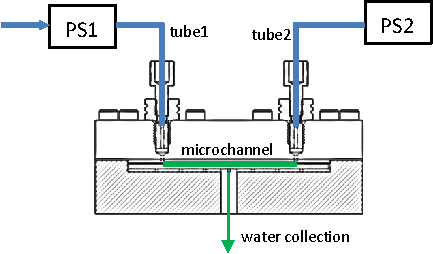
\includegraphics[width=0.55\textwidth]{figures/packagingandtestunderhighpressure/figure4_20}%
\caption{Schematic setup of permeate flux measurement of dead end.}%
\label{figure4_20}%
\end{figure}

To test the permeability the volumetric flow rate is measured when pressurized to certain pressure. This is realized by measuring the mass of the water collected at the permeation flow outlet. \autoref{figure4_21} shows the total collected volume of water and the corresponding flow rate versus time. The mass of the harvested water is recorded every 10 seconds right after it is pressurize to 7.4bar for 20 minutes since the permeate flux is relatively large in the beginning, then it is recorded every 2 minutes. The total recording time is 135 minutes.\\

\begin{figure}[ht]%
\centering
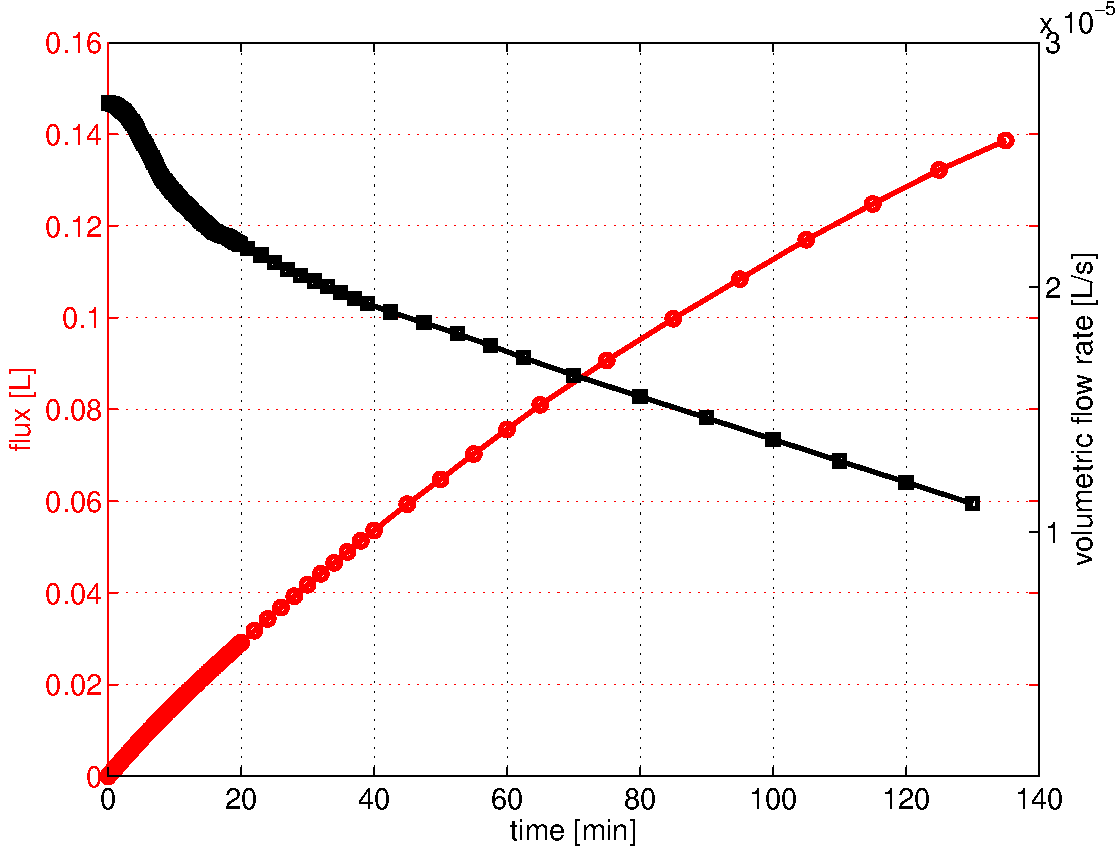
\includegraphics[width=0.6\textwidth]{figures/packagingandtestunderhighpressure/figure4_21.pdf}%
\caption{Deionized water permeate flux with dead end and corresponding permeation flow rate with respect to time.}%
\label{figure4_21}%
\end{figure}

The permeate flow rate reaches the peak at the beginning and decreases with time. However, it decreases continuously afterwards. This phenomenon happens because of the NF membrane compaction. Membrane compaction is an irreversible phenomenon that when the NF membrane is put under pressure, the polymers are slightly reorganized and the structure is changed, resulting in a lowered volume porosity, increased membrane resistance and eventually lowered flux \cite{persson1995study}. If no membrane compaction occurred, the flux would have a linear correlation with pressure and the flow rate will be constant as well. Since the mass flow rate profile in \autoref{figure4_21} presents a continuous linear decrease, the compacting process of the NF membrane does not end within two hours. \autoref{equation4_11} gives the calculation formula of the membrane permeability \cite{waterpermeaility}:

\begin{equation}
    L_p = \frac{I_V}{A\cdot \Delta P}
    \label{equation4_11}
\end{equation}

The membrane permeability defined by the above equation is the volumetric flow rate over contact area and the pressure difference. $I_V$ is the volumetric flow rate and $A$ is the contact area. J.F. Fernandez et al. provided the test data for the permeability of pure water permeability of this compacted NF membrane, which was 4.6L/m$^2$hbar \cite{fernandez2011thinking}. \autoref{figure4_22} shows the change of membrane permeability with respect to time. During the compacting of the membrane the permeability decreases linearly and eventually it will reach a steady state, which is the permeability of compacted membrane. In this master thesis this is not tested due to time limit.\\

\clearpage

\begin{figure}[ht]%
\centering
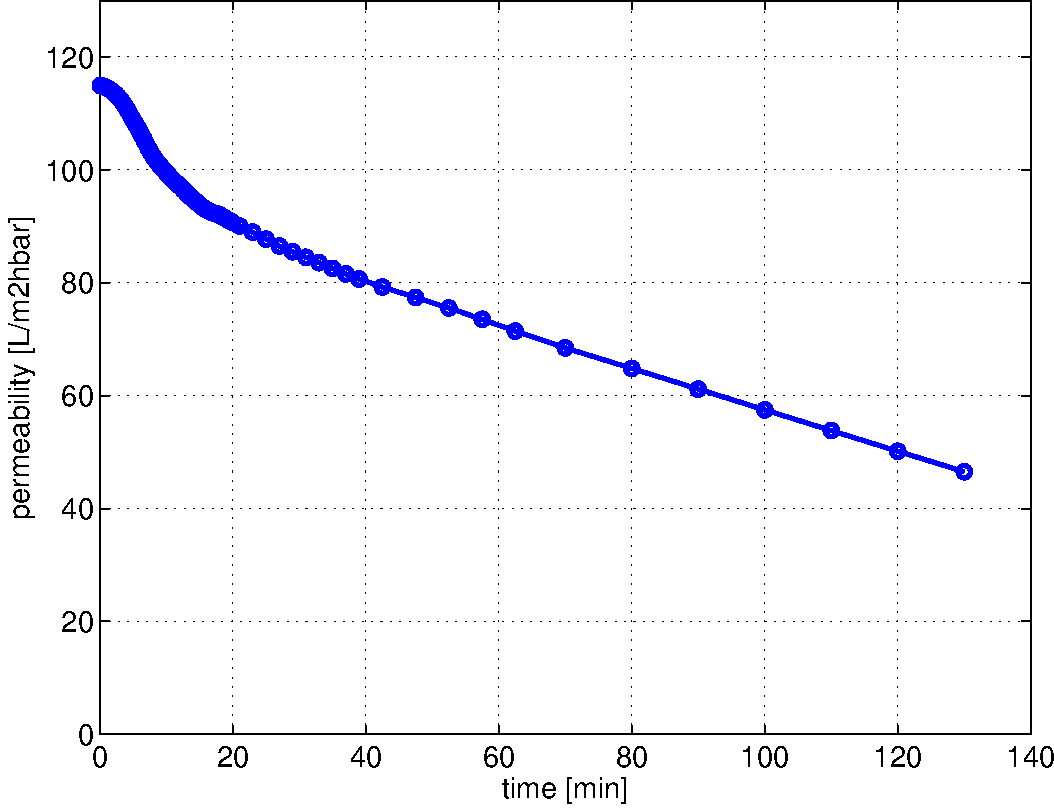
\includegraphics[width=0.6\textwidth]{figures/packagingandtestunderhighpressure/figure4_22.pdf}%
\caption{Deionized water permeability profile of uncompacted NF membrane with respect to time.}%
\label{figure4_22}%
\end{figure}

\noindent \textit{Sodium chloride solution permeability of the NF membrane}\\

With the former test setup the sodium chloride solution permeability is also tested under the same pressure (7.4bar) for two times. The concentration of the sodium chloride in deionized water is 5g/L. The test conducted is with non-compacted NF membrane.\\

\autoref{figure4_23} shows the flux harvested at the permeation outlet interface versus time and the corresponding permeation volumetric flow rate. The permeation flow rate of the both tests reached the peak at the beginning and decreased with time. After about five hours the permeation flow rate tended to become constant. This is perhaps because the compacting process of the NF membrane is going to end then. The flux curve of the both tests did not vary much while the permeate flow rate of the second test was a bit higher than the first test when they reached the steady value. The permeability curve shown in \autoref{figure4_24} has the same tendency as the permeation flow rate. This sodium chloride solution permeation flux and the permeability of uncompacted NF membrane is much smaller compared to the deionized water permeability of uncompacted NF membrane shown in \autoref{figure4_22}. This is due to the osmotic pressure difference accross the NF membrane since most of the salt ions will be rejected by the NF membrane. \autoref{equation4_14} give the influence of the osmotic pressure upon the permeate flux \cite{ref_5}.

\begin{equation}
    J_v=A(\Delta P-\Delta \pi _w)
    \label{equation4_14}
\end{equation}

In the above equation, $J_v$ is the fluid flux through the NF membrane. $A$ is the membrane permeability constant which is the pure water membrane permeability, $L_p$. $\Delta P$ is the driving pressure across the membrane and $\Delta \pi _w$ is the osmotic pressure difference across the membrane. When the water in the NaCl solution permeate through the membrane and the salt ions are rejected, the concentration of salt will increase at the membrane surface, leading to the increase of the osmotic pressure and thus the decrease of the permeation flux based on \autoref{equation4_14}. This osmotic pressure will then increase to a saturation state, which will cause a equilibrium between the driving pressure and the osmotic pressure, resulting in a constant permeation flow rate as shown in \autoref{figure4_24}. For further studies the conductivity of the collected solution both from the permeation flow and the cross flow could be measured in order to calculate the salt rejection ratio of this NF membrane.

\begin{figure}[!t]%
\centering
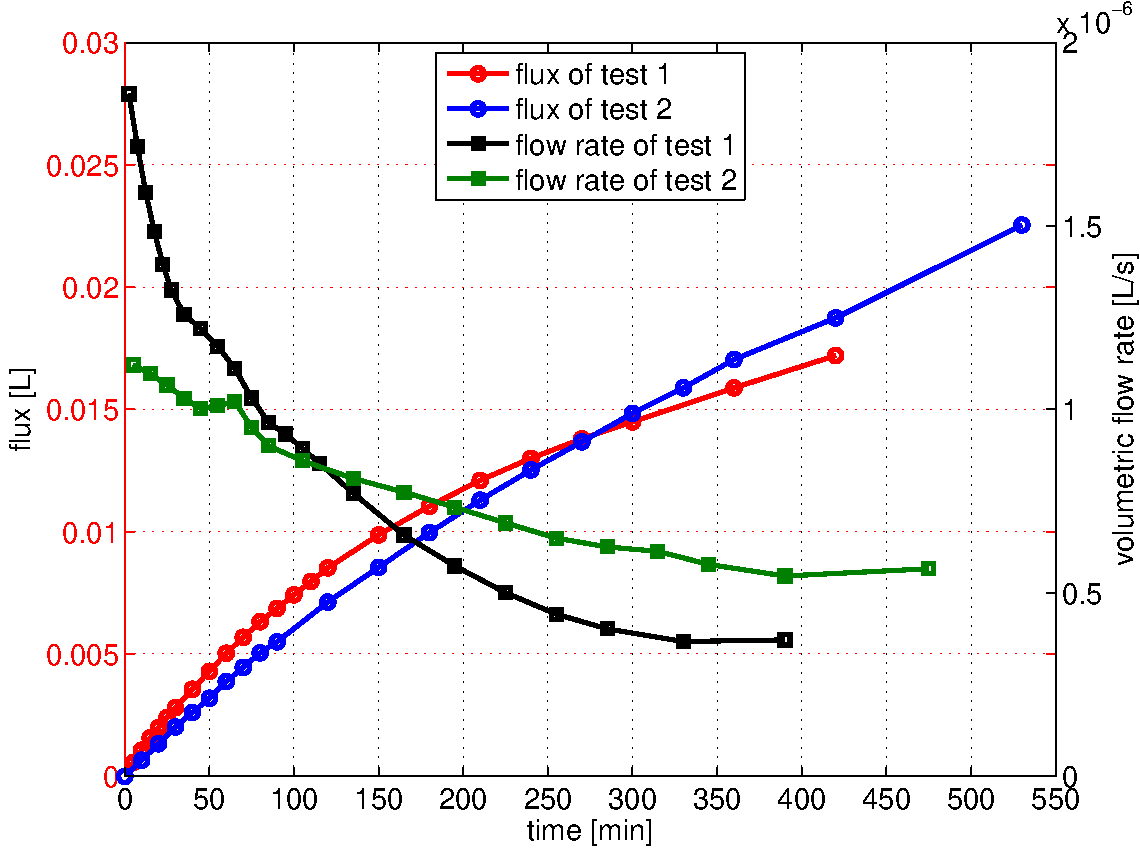
\includegraphics[width=0.6\textwidth]{figures/packagingandtestunderhighpressure/figure4_25.pdf}%
\caption{Sodium chloride solution permeate flux with uncompacted NF membrane and corresponding permeation flow rate with respect to time.}%
\label{figure4_23}%
\end{figure}

\begin{figure}[ht]%
\centering
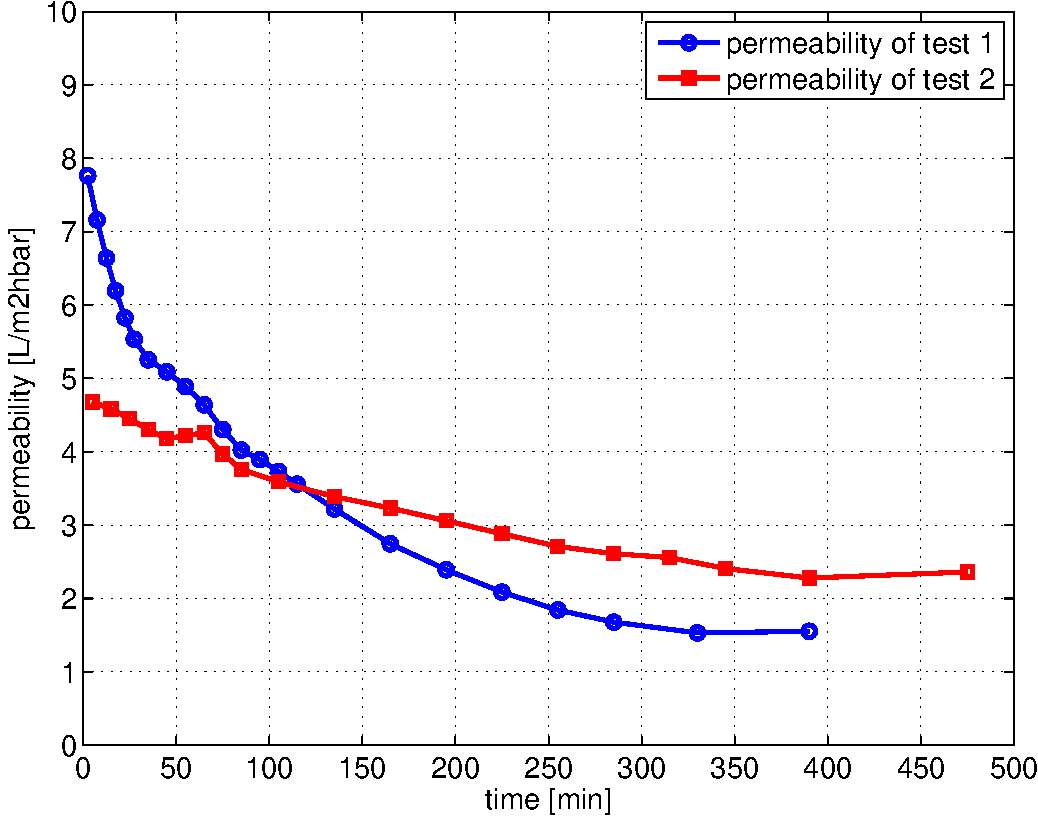
\includegraphics[width=0.54\textwidth]{figures/packagingandtestunderhighpressure/figure4_26.pdf}%
\caption{Sodium chloride solution permeability profile of uncompacted NF membrane with respect to time.}%
\label{figure4_24}%
\end{figure}

\clearpage

